
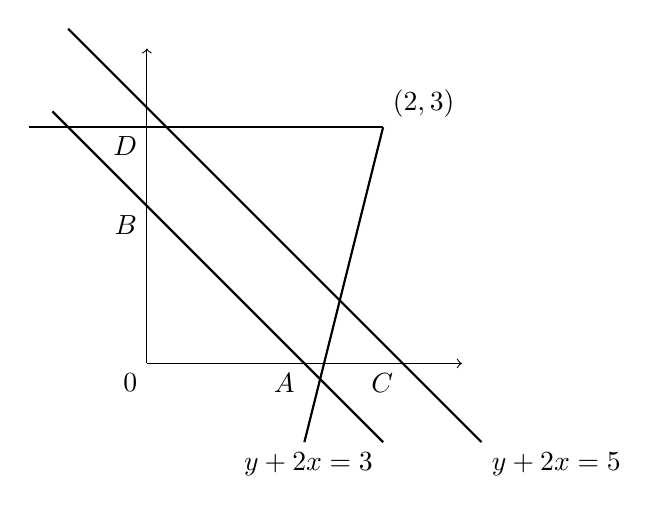
\begin{tikzpicture}
\draw[->] (0,0) -- (4,0) node[right] {};
\draw[->] (0,0) -- (0,4) node[above] {};


\draw[thick] (-1,4.25) -- (4.25,-1) node[below right] {$y + 2x = 5$};
\draw[thick] (-1.2,3.2) -- (3,-1) node[below left] {$y + 2x = 3$};


\filldraw[black] (0,0)  node[below left] {$0$};
\filldraw[black] (2,0)  node[below left] {$A$};
\filldraw[black] (3.25,0)  node[below left] {$C$};
\filldraw[black] (3,3)  node[above right] {$(2,3)$};


\draw[thick] (-1.5,3) -- (3,3) node[midway, right] {};

\draw[thick] (2,-1) -- (3,3) node[midway, right] {};


\node[below left ] at (0,2) {$B$};
\node[below left ] at (-0,3) {$D$};
\end{tikzpicture}

